\section{Podstawy teoretyczne i przegląd rozwiązań}
\subsection{Sieć neuronowa}
Sieć neuronowa to model matematyczny inspirowany działaniem mózgu.
Składa się z sztucznych neuronów (dalej nazywanych neuronami)
oraz synapsów (w terminologi angielskiej występują one pod nazwą \textit{edges}).

\noindent\\
Obecnie sieci neuronowe są mocno rozwijanym działem informatyki.
Z tego powodu powstało wiele typów sieci,
które można uogólnić do kategorii jednokierunkowej sieci neuronowej
(ang. \textit{feedforward neural networks})
oraz rekurencyjnej sieci neuronowej (ang. \textit{recurrent neural networks}).
W angielskiej literaturze można spotkać jeszcze następujące typy sieci:
recursive neural network, feedback neural network.
W niniejszym dokumencie sieci neuronowe odnoszą się
do jednokierunkowej sieci neuronowej (FNN),
a dokładniej do jej szczególnego przypadku nazwanego
wielowarstwowym perceptronem (ang. \textit{multilayer perceptron}).
Jego cechą charakterystyczną jest brak synapsów między warstwami,
które nie są "obok siebie".
Oznacza to, że obie poniższe sieci są jednokierunkowe,
ale tylko ta po prawej jest wielowarstwowym perceptronem (MLP):

\noindent
\begin{center}
  
\includegraphics[trim={0 0 0 0}, height=6.5cm, clip]{sections/02_img/fnn.png}
  \hspace{2cm}
  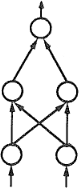
\includegraphics[trim={0 0 0 0}, height=6.5cm, clip]{sections/02_img/fnn_mlp.png}
\end{center}

\noindent
W MLP można wyróżnić trzy rodzaje warstw: wejściowe, ukryte i wyjściowe.
Ponieważ wejściowa warstwa musi być wielkości danych wejściowych,
a warstwa wyjściowa - danych wyjściowych,
to~zmienne są tylko warstwy ukryte i to ich połączenia można optymalizować.

\subsubsection*{Architektura sieci neuronowej}
Architektura sieci, w rozumieniu niniejszego dokumentu,
to: liczba warstw ukrytych, liczba neuronów w każdej z warstw,
i funkcja aktywacji każdej z warstw.

\noindent\\
Nie zalicza się natomiast do niej liczby synapsów,
ponieważ warstwy są między sobą w pełni połą\-czone.
Nie zalicza się również do architektury wag synapsów
- są określane w procesie ucze\-nia~się.
Z~tego powodu nie są częścią architektury,
a procesu oceniania jej przystosowania.

\subsection{Podejście genetyczne do rozwijania architektury}
Algorytmem, który zostanie wykorzystany do optymalizacji
architektury sieci neuronowej, jest algorytm genetyczny.
Opiera się on na mechanizmie zaobserwowanym w przyrodzie,
zwanym ewolucją, gdzie poprzez krzyżowanie i mutację
następuje powstawanie nowych osobników,
które całościowo jako populacja są coraz lepiej przystosowane.

\subsection{Przegląd rozwiązań}
% https://arxiv.org/abs/2003.06505
% https://arxiv.org/pdf/2003.06505
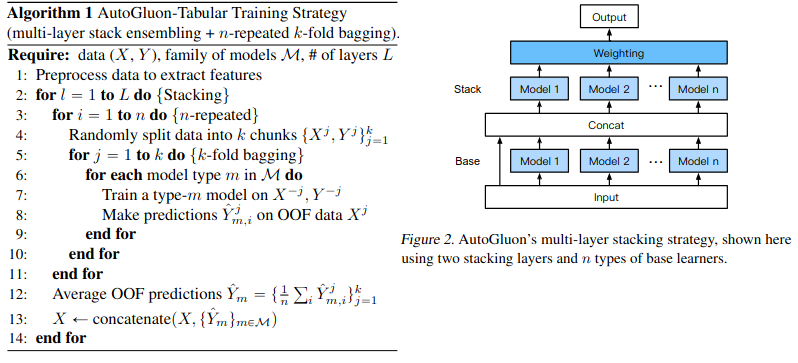
\includegraphics[width=\textwidth,clip]{sections/02_img/AutoGluon.png}
% https://dl.acm.org/doi/10.1145/3292500.3330648
% https://dl.acm.org/doi/epdf/10.1145/3292500.3330648
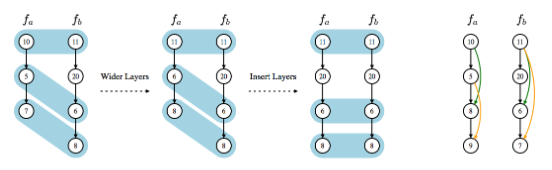
\includegraphics[width=\textwidth,clip]{sections/02_img/AutoKeras.png}
